\section{Hasil tiap mitra}\label{sec:bilateral}

\subsection{Gambaran umumnya}

Hasil total tiap mitra berbeda. Australia dan Malaysia memberi NARDL yang lebih mendukung, tetapi signifikansi Malaysia lebih lemah setelah BH. Model lain tetap ditampilkan, termasuk yang mempunyai koefisien besar atau p-value kecil tetapi belum lolos pemeriksaan long run.

\begin{table}[!htbp]\centering\caption{Ringkasan NARDL Indonesia dengan sepuluh mitra}{\small\setlength{\tabcolsep}{3pt}\renewcommand{\arraystretch}{1.15}
\begin{tabular}{p{0.17\linewidth}p{0.045\linewidth}p{0.2\linewidth}p{0.12\linewidth}p{0.09\linewidth}p{0.09\linewidth}p{0.07\linewidth}}
\toprule
\textbf{Mitra} & \textbf{N} & \textbf{Rentang} & \textbf{Koef. dep.} & \textbf{p} & \textbf{BH} & \textbf{Status}\\
\midrule
Australia & 77 & 2007Q1--2026Q1 & 3,356 & \(<0{,}001\) & 0,004 & L+D\\
Tiongkok & 78 & 2007Q1--2026Q2 & -2,727 & 0,250 & 0,350 & --\\
India & 49 & 2014Q1--2026Q1 & -6,443 & 0,236 & 0,350 & --\\
Jepang & 78 & 2007Q1--2026Q2 & -2,456 & 0,006 & 0,020 & --\\
Korea Selatan & 78 & 2007Q1--2026Q2 & 3,935 & 0,144 & 0,288 & --\\
Malaysia & 78 & 2007Q1--2026Q2 & 1,346 & 0,024 & 0,059 & L+D\\
Singapura & 78 & 2007Q1--2026Q2 & -0,262 & 0,810 & 0,810 & --\\
Thailand & 78 & 2007Q1--2026Q2 & 0,950 & 0,280 & 0,350 & L\\
Amerika Serikat & 75 & 2007Q1--2025Q3 & 3,095 & 0,006 & 0,020 & --\\
Vietnam & 74 & 2007Q1--2025Q2 & -0,551 & 0,737 & 0,810 & --\\
\bottomrule
\end{tabular}
}\label{tab:bilateral}\end{table}

\begin{figure}[!htbp]\centering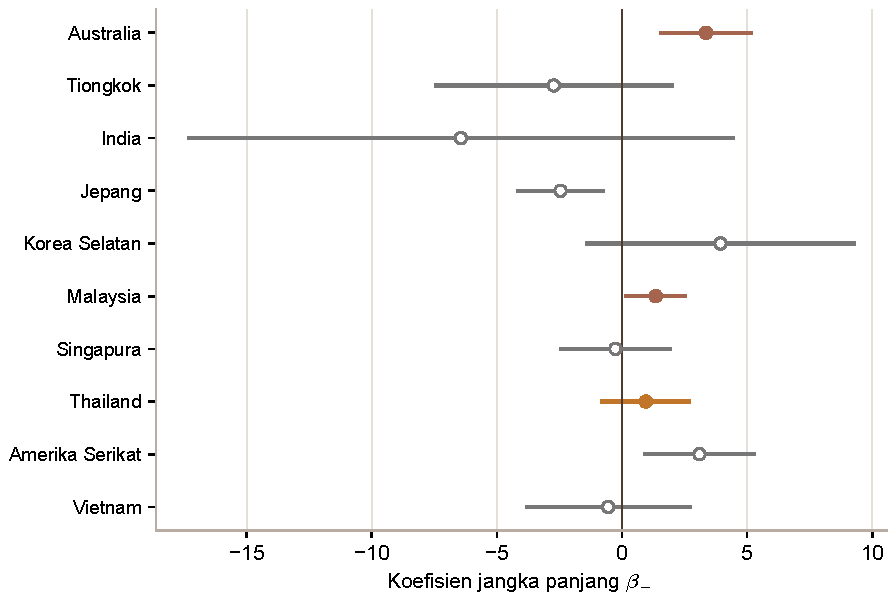
\includegraphics[width=\linewidth]{assets/bilateral_forest.pdf}\caption{Koefisien depresiasi NARDL. Cokelat: long run dan diagnostic tests terpenuhi; emas: ada catatan model; simbol kosong: bukti long run belum cukup.}\label{fig:bilateralforest}\end{figure}


Periode data tiap mitra tidak sama. Karena itu, perbedaan koefisien belum menjadi uji formal bahwa negara-negara tersebut mempunyai efek yang berbeda.

\clearpage\subsection{Indonesia--Australia}

Australia termasuk hasil yang lebih mendukung perbaikan rasio perdagangan saat rupiah melemah. ARDL dan NARDL sama-sama lolos pemeriksaan utama. Pada NARDL, signifikansi koefisien depresiasi juga bertahan setelah BH.

Garis NARDL memburuk dahulu lalu membaik, sehingga ada pola J pada garis utama. Tetapi confidence interval awal masih melewati nol. Jadi, pemburukan awalnya belum sekuat kepastian yang terlihat dari garis saja. Uji asymmetry juga belum menolak kesamaan kedua arah kurs pada 5\%.

\noindent\textbf{Angka utamanya.} NARDL memakai 77 kuartal pada 2007Q1--2026Q1. Koefisien depresiasi 3,356, confidence interval 95\% [1,563; 5,149], p-value \(<0{,}001\), dan BH 0,004. P-value asymmetry 0,147.

\noindent\textbf{Catatan pemeriksaan.} tidak ada masalah yang terdeteksi pada pemeriksaan yang dipakai.

\begin{figure}[!htbp]\centering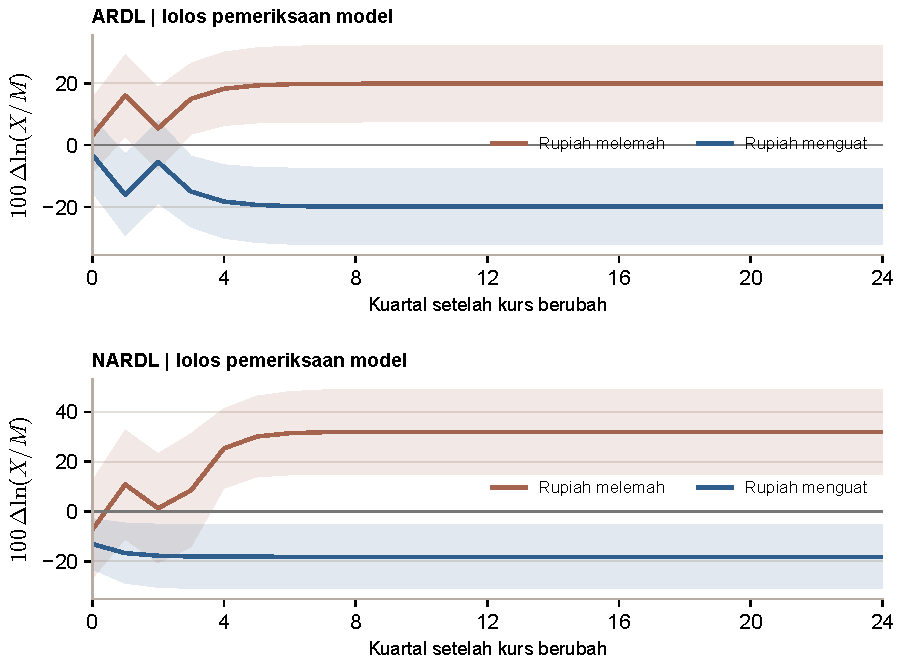
\includegraphics[width=\linewidth]{assets/response_BIL_AUS.pdf}\caption{Respons perdagangan Indonesia--Australia. Positif berarti rasio ekspor/impor membaik. Confidence interval berlaku per horizon; skala panel berbeda.}\label{fig:bilAUS}\end{figure}


\clearpage\subsection{Indonesia--Tiongkok}

Besarnya perdagangan dengan Tiongkok belum membuat hasil modelnya lebih pasti. Kedua model total bilateral belum lolos pemeriksaan long run. NARDL mempunyai catatan autocorrelation, sedangkan ARDL mendapat catatan CUSUM.

Karena itu, tanda negatif belum cukup untuk menyimpulkan bahwa depresiasi merugikan seluruh perdagangan Indonesia dengan Tiongkok. Kelompok pertanian nantinya memberi hasil yang berbeda dan lebih mendukung. Defisit bilateral pada data tahunan juga belum membuktikan bahwa kurs adalah penyebabnya.

\noindent\textbf{Angka utamanya.} NARDL memakai 78 kuartal pada 2007Q1--2026Q2. Koefisien depresiasi -2,727, confidence interval 95\% [-7,427; 1,972], p-value 0,250, dan BH 0,350. P-value asymmetry 0,905.

\noindent\textbf{Catatan pemeriksaan.} bounds test belum memberi bukti yang cukup; joint-X test belum mendukung; ada catatan pada residual atau stabilitas model.

\begin{figure}[!htbp]\centering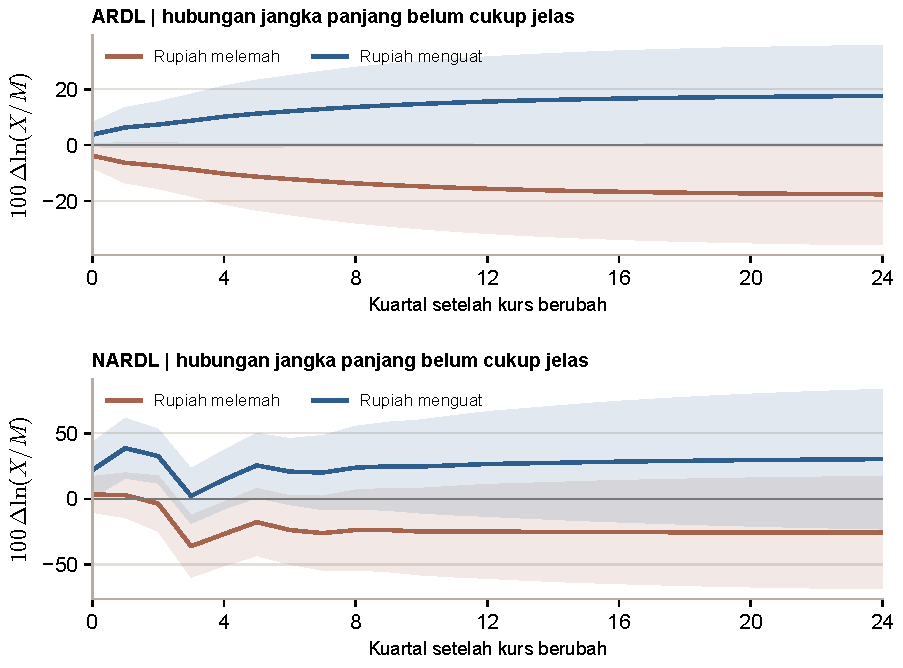
\includegraphics[width=\linewidth]{assets/response_BIL_CHN.pdf}\caption{Respons perdagangan Indonesia--Tiongkok. Positif berarti rasio ekspor/impor membaik. Confidence interval berlaku per horizon; skala panel berbeda.}\label{fig:bilCHN}\end{figure}


\clearpage\subsection{Indonesia--India}

India mempunyai data lebih pendek karena baseline memakai CPI mulai 2013. Dengan lebih banyak parameter pada NARDL, informasi untuk masing-masing angka menjadi terbatas. Koefisien depresiasinya negatif, tetapi confidence interval lebar dan bounds test belum mendukung long run.

Uji asymmetry signifikan, tetapi itu belum menyelesaikan persoalan bounds test. Diagnostic tests NARDL tidak menemukan masalah yang diperiksa, sedangkan ARDL mempunyai catatan autocorrelation dan RESET. WPI hanya dipakai sebagai pembanding terpisah, bukan dianggap CPI yang sama.

\noindent\textbf{Angka utamanya.} NARDL memakai 49 kuartal pada 2014Q1--2026Q1. Koefisien depresiasi -6,443, confidence interval 95\% [-17,300; 4,414], p-value 0,236, dan BH 0,350. P-value asymmetry 0,021.

\noindent\textbf{Catatan pemeriksaan.} bounds test belum memberi bukti yang cukup; joint-X test belum mendukung.

\begin{figure}[!htbp]\centering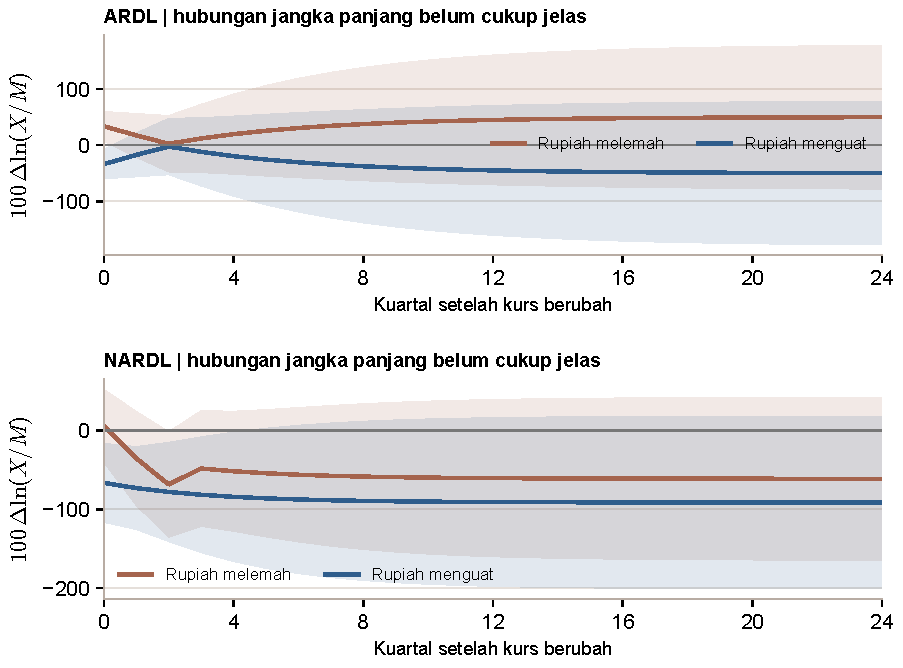
\includegraphics[width=\linewidth]{assets/response_BIL_IND.pdf}\caption{Respons perdagangan Indonesia--India. Positif berarti rasio ekspor/impor membaik. Confidence interval berlaku per horizon; skala panel berbeda.}\label{fig:bilIND}\end{figure}


\clearpage\subsection{Indonesia--Jepang}

Jepang memberi contoh mengapa p-value koefisien tidak boleh dibaca sendirian. Koefisien depresiasi NARDL negatif dan signifikan, termasuk setelah BH. Tetapi F bounds dan t bounds belum sama-sama memenuhi aturan 5\%.

Ada pula catatan ARCH dan normality test. Jadi, hasil ini tetap dilaporkan tetapi belum dipakai sebagai kesimpulan long run yang kuat. Tanda negatifnya adalah temuan yang perlu ditinjau lebih lanjut, bukan bukti pasti bahwa ekspor Indonesia ke Jepang turun karena depresiasi.

\noindent\textbf{Angka utamanya.} NARDL memakai 78 kuartal pada 2007Q1--2026Q2. Koefisien depresiasi -2,456, confidence interval 95\% [-4,166; -0,747], p-value 0,006, dan BH 0,020. P-value asymmetry 0,971.

\noindent\textbf{Catatan pemeriksaan.} bounds test belum memberi bukti yang cukup; ada catatan pada residual atau stabilitas model.

\begin{figure}[!htbp]\centering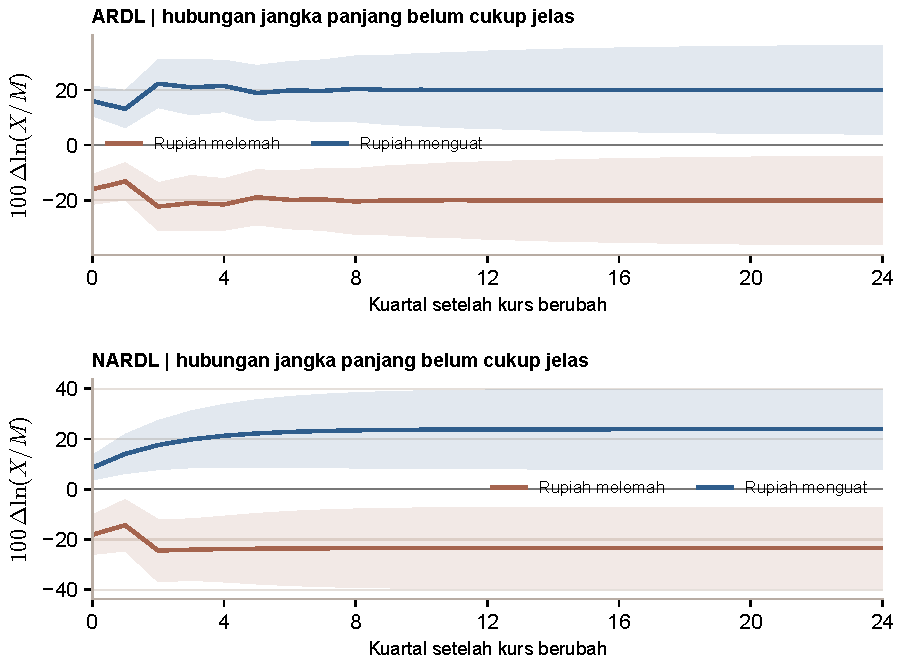
\includegraphics[width=\linewidth]{assets/response_BIL_JPN.pdf}\caption{Respons perdagangan Indonesia--Jepang. Positif berarti rasio ekspor/impor membaik. Confidence interval berlaku per horizon; skala panel berbeda.}\label{fig:bilJPN}\end{figure}


\clearpage\subsection{Indonesia--Korea Selatan}

Koefisien depresiasi NARDL Korea positif, tetapi cukup tidak pasti. Pemeriksaan long run belum lengkap, dan ada catatan autocorrelation, RESET, serta CUSUM. ARDL lebih dekat ke nol, tetapi juga belum mendukung long run.

Pada kelompok modal, hasil NARDL justru lebih mendukung dan pola J lebih jelas. Ini memperlihatkan bahwa hasil total mitra bisa menutupi kelompok tertentu. Namun barang modal tetap hanya sebagian perdagangan Indonesia dengan Korea.

\noindent\textbf{Angka utamanya.} NARDL memakai 78 kuartal pada 2007Q1--2026Q2. Koefisien depresiasi 3,935, confidence interval 95\% [-1,383; 9,253], p-value 0,144, dan BH 0,288. P-value asymmetry 0,112.

\noindent\textbf{Catatan pemeriksaan.} bounds test belum memberi bukti yang cukup; joint-X test belum mendukung; ada catatan pada residual atau stabilitas model.

\begin{figure}[!htbp]\centering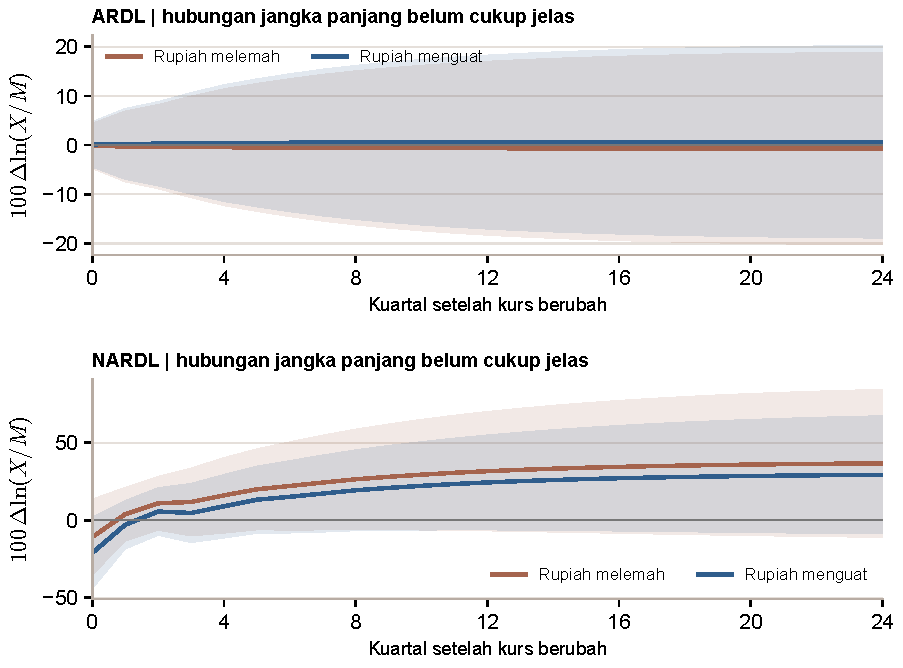
\includegraphics[width=\linewidth]{assets/response_BIL_KOR.pdf}\caption{Respons perdagangan Indonesia--Korea Selatan. Positif berarti rasio ekspor/impor membaik. Confidence interval berlaku per horizon; skala panel berbeda.}\label{fig:bilKOR}\end{figure}


\clearpage\subsection{Indonesia--Malaysia}

Malaysia memperlihatkan perbedaan ARDL dan NARDL yang cukup besar. ARDL mendukung long run, tetapi koefisien kursnya negatif, tidak signifikan pada 5\%, dan ada catatan RESET serta CUSUM. NARDL memberi koefisien depresiasi positif dan lolos pemeriksaan utama.

P-value depresiasi NARDL sekitar 0,024, tetapi setelah BH sekitar 0,059. Jadi, signifikansinya tidak bertahan pada ambang 5\% setelah koreksi tersebut. Kurva yang membaik juga belum tentu J-curve jika tidak mempunyai fase awal memburuk.

\noindent\textbf{Angka utamanya.} NARDL memakai 78 kuartal pada 2007Q1--2026Q2. Koefisien depresiasi 1,346, confidence interval 95\% [0,186; 2,507], p-value 0,024, dan BH 0,059. P-value asymmetry \(<0{,}001\).

\noindent\textbf{Catatan pemeriksaan.} tidak ada masalah yang terdeteksi pada pemeriksaan yang dipakai.

\begin{figure}[!htbp]\centering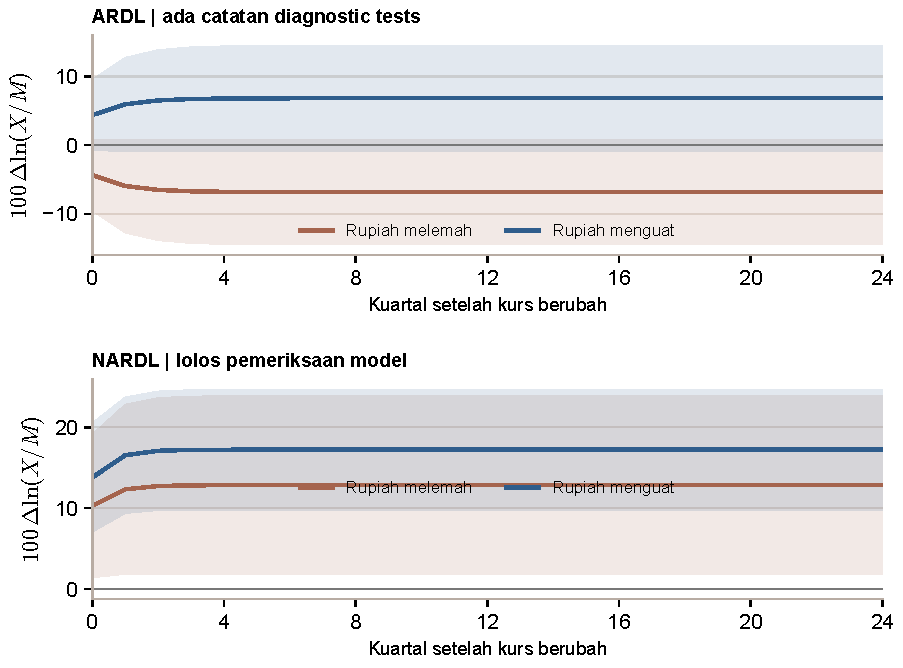
\includegraphics[width=\linewidth]{assets/response_BIL_MYS.pdf}\caption{Respons perdagangan Indonesia--Malaysia. Positif berarti rasio ekspor/impor membaik. Confidence interval berlaku per horizon; skala panel berbeda.}\label{fig:bilMYS}\end{figure}


\clearpage\subsection{Indonesia--Singapura}

Pada Singapura, F dan t bounds dapat menolak sementara joint-X test belum mendukung. Artinya, aturan lengkap untuk membaca long run belum terpenuhi. ARDL menunjukkan bahwa diagnostic tests yang tidak menemukan masalah belum cukup jika pemeriksaan long run lainnya belum lolos.

Koefisien depresiasi NARDL dekat nol pada garis utama, tetapi intervalnya tetap perlu dilihat. Kita belum bisa menyebutnya tidak sensitif karena belum ada uji khusus untuk memastikan efeknya kecil.

\noindent\textbf{Angka utamanya.} NARDL memakai 78 kuartal pada 2007Q1--2026Q2. Koefisien depresiasi -0,262, confidence interval 95\% [-2,440; 1,915], p-value 0,810, dan BH 0,810. P-value asymmetry 0,791.

\noindent\textbf{Catatan pemeriksaan.} joint-X test belum mendukung; ada catatan pada residual atau stabilitas model.

\begin{figure}[!htbp]\centering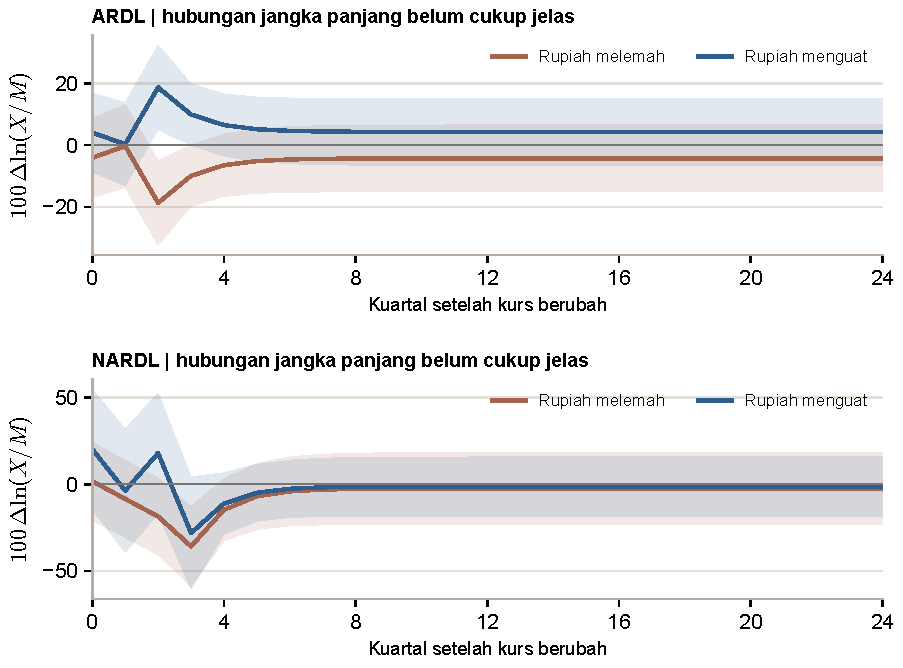
\includegraphics[width=\linewidth]{assets/response_BIL_SGP.pdf}\caption{Respons perdagangan Indonesia--Singapura. Positif berarti rasio ekspor/impor membaik. Confidence interval berlaku per horizon; skala panel berbeda.}\label{fig:bilSGP}\end{figure}


\clearpage\subsection{Indonesia--Thailand}

Thailand mempunyai dukungan long run pada kedua model. Tetapi ARCH dan CUSUMSQ memberi catatan, dengan tambahan CUSUM pada NARDL. Koefisien depresiasi NARDL juga belum signifikan.

Kurs Thailand mempunyai catatan perbedaan definisi antarpenyedia. Seri GEM dipakai sebagai robustness check secara penuh, bukan untuk menambal satu angka baseline. Perbandingan sumber perlu memperhatikan definisi dan periode data. Hasilnya belum menjadi efek kebijakan yang pasti stabil.

\noindent\textbf{Angka utamanya.} NARDL memakai 78 kuartal pada 2007Q1--2026Q2. Koefisien depresiasi 0,950, confidence interval 95\% [-0,789; 2,690], p-value 0,280, dan BH 0,350. P-value asymmetry 0,765.

\noindent\textbf{Catatan pemeriksaan.} ada catatan pada residual atau stabilitas model.

\begin{figure}[!htbp]\centering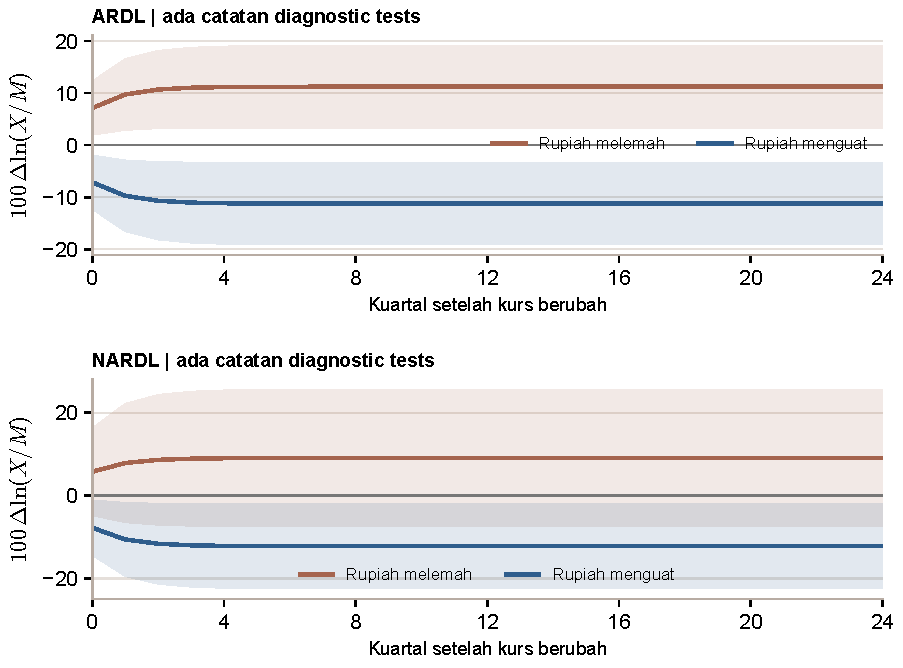
\includegraphics[width=\linewidth]{assets/response_BIL_THA.pdf}\caption{Respons perdagangan Indonesia--Thailand. Positif berarti rasio ekspor/impor membaik. Confidence interval berlaku per horizon; skala panel berbeda.}\label{fig:bilTHA}\end{figure}


\clearpage\subsection{Indonesia--Amerika Serikat}

Koefisien depresiasi NARDL AS positif dan signifikan, termasuk setelah BH. F dan t bounds juga menolak. Tetapi joint-X sekitar 0,060 belum memenuhi ambang 5\%, sehingga aturan long run lengkap belum terpenuhi. Ada pula catatan CUSUMSQ dan normality test.

Sampel utama berhenti pada 2025Q3 karena CPI Oktober 2025 kosong pada seri yang dipakai. Kelompok konsumsi dengan AS memberi hasil berbeda dan pola J lebih jelas. Itu belum memperbaiki kelemahan model total karena barang yang dihitung berbeda.

\noindent\textbf{Angka utamanya.} NARDL memakai 75 kuartal pada 2007Q1--2025Q3. Koefisien depresiasi 3,095, confidence interval 95\% [0,921; 5,269], p-value 0,006, dan BH 0,020. P-value asymmetry 0,240.

\noindent\textbf{Catatan pemeriksaan.} joint-X test belum mendukung; ada catatan pada residual atau stabilitas model.

\begin{figure}[!htbp]\centering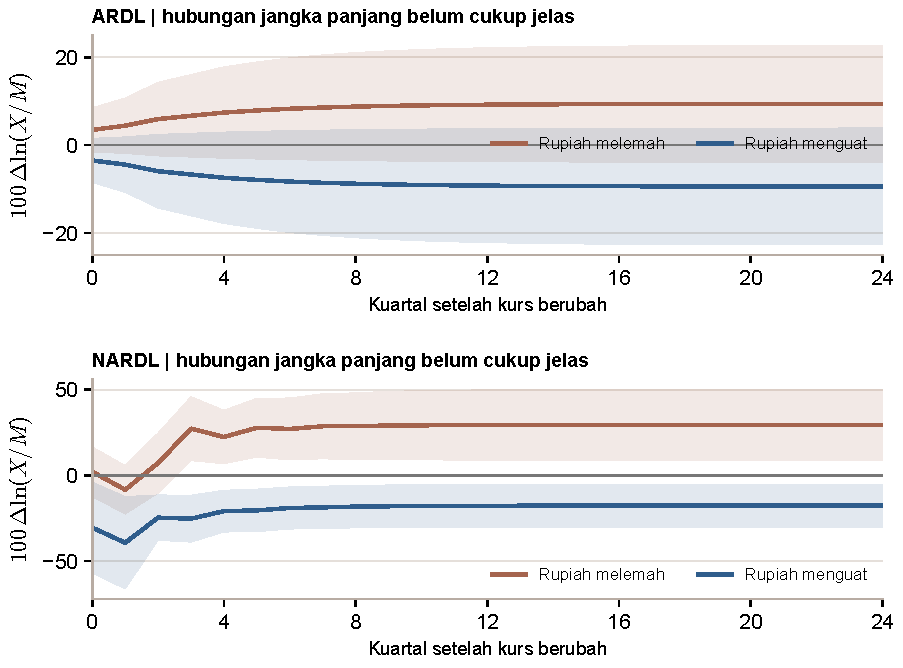
\includegraphics[width=\linewidth]{assets/response_BIL_USA.pdf}\caption{Respons perdagangan Indonesia--Amerika Serikat. Positif berarti rasio ekspor/impor membaik. Confidence interval berlaku per horizon; skala panel berbeda.}\label{fig:bilUSA}\end{figure}


\clearpage\subsection{Indonesia--Vietnam}

Vietnam mempunyai beberapa catatan variasi residual dan stabilitas. Koefisien depresiasi NARDL negatif dan tidak signifikan. T bounds juga belum mendukung long run. ARDL pun belum lolos pemeriksaan lengkap.

Kurs Agustus 2025 yang kosong membuat rentang utama berakhir pada 2025Q2. Kuartal setelah celah tidak disambung seolah tidak ada jeda. Alternatif GEM menjadi robustness check tersendiri. Keterbatasan ini perlu diingat saat membandingkan Vietnam dengan negara yang datanya berakhir lebih akhir.

\noindent\textbf{Angka utamanya.} NARDL memakai 74 kuartal pada 2007Q1--2025Q2. Koefisien depresiasi -0,551, confidence interval 95\% [-3,806; 2,704], p-value 0,737, dan BH 0,810. P-value asymmetry 0,163.

\noindent\textbf{Catatan pemeriksaan.} bounds test belum memberi bukti yang cukup; ada catatan pada residual atau stabilitas model.

\begin{figure}[!htbp]\centering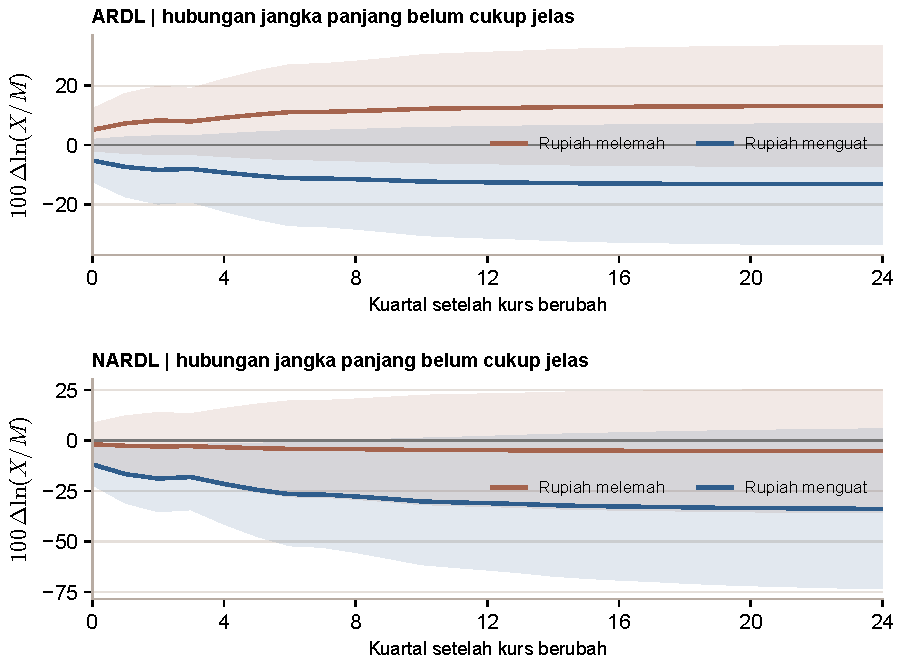
\includegraphics[width=\linewidth]{assets/response_BIL_VNM.pdf}\caption{Respons perdagangan Indonesia--Vietnam. Positif berarti rasio ekspor/impor membaik. Confidence interval berlaku per horizon; skala panel berbeda.}\label{fig:bilVNM}\end{figure}
